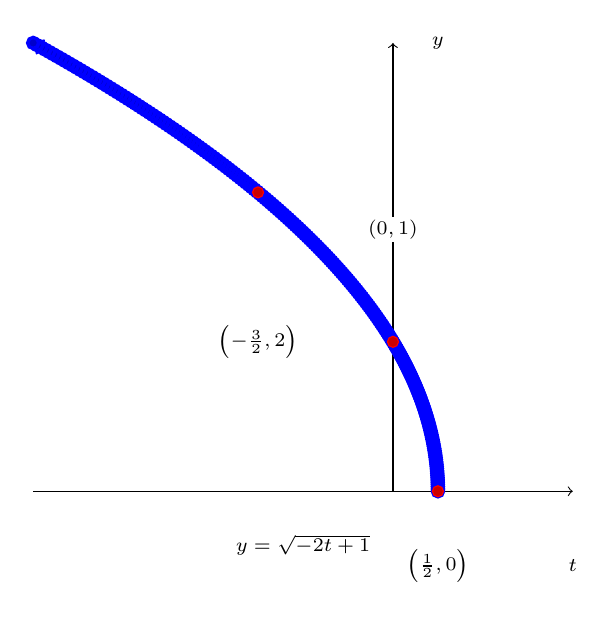
\begin{tikzpicture}
\begin{axis}[
  xmin=-4, xmax=2,
  ymin=0, ymax=3,
  axis lines=middle,
  axis line style={->},
  ticks=none,
  clip=false
]
\node at (axis cs:2,-0.5){\scriptsize $t$};
\node at (axis cs:0.5,3){\scriptsize $y$};
\node at (axis cs:0.5,-0.5){\scriptsize $\left(\frac{1}{2},0 \right)$};
% Emulating gclear with a white background for the label
\node[fill=white, inner sep=1pt] at (axis cs:0,1.75){\scriptsize $(0,1)$};
\node at (axis cs:-1.5,1){\scriptsize $\left(-\frac{3}{2},2 \right)$};

\addplot+[domain=0:3, samples=200, smooth, line width=1.25pt, ->, variable=\t, parametric]
  ({( (\t^2-1)/(-2) )},{\t});

\addplot+[only marks, mark=*, mark size=2pt] coordinates {(0.5,0) (0,1) (-1.5,2)};

% Caption
\node at (rel axis cs:0.5,-0.12){\scriptsize $y=\sqrt{-2t+1}$};
\end{axis}
\end{tikzpicture}